\hsectionENDE{Airline Example}{Fluglienen-Beispiel}%
%
\begin{figure}%
\centering%
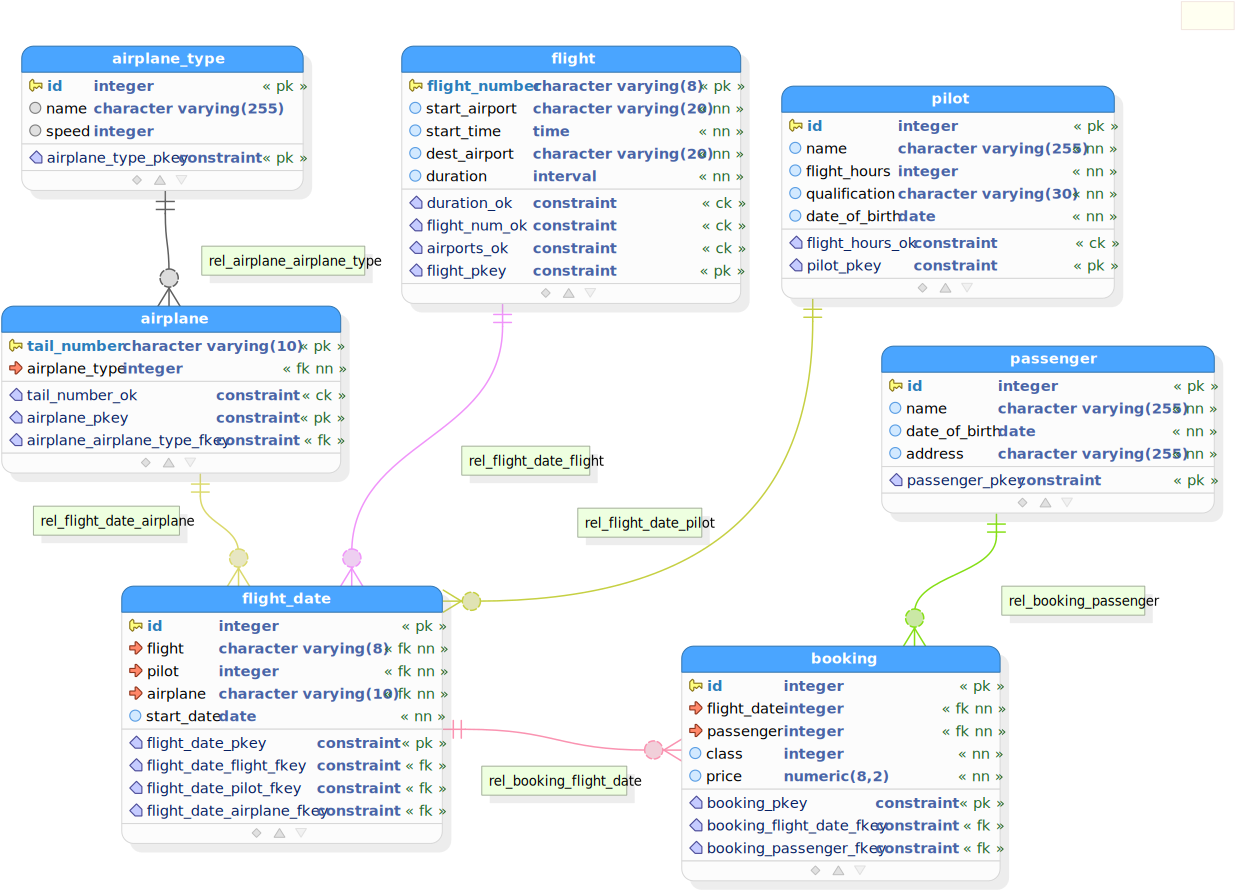
\includegraphics[width=0.95\linewidth]{\currentDir/airline}%
\caption{The logical model of the airline example. Das logische Modell des Airline-Beispiels.}%
\label{fig:airline}%
\end{figure}%
%
\qENDE{%
 Now we look at a larger consistent example. %
The logical model of an airline \db\ is given in \cref{fig:airline}.%
}{%
Jetzt schauen wir uns ein größeres, konsistentes Beispiel an. %
Das logische Modell einer Airline-Datenbank ist in \cref{fig:airline} gegeben.%
}%
%
\begin{questionENDE}{Database Creation}{Datenbank Erstellen}%
\gitLoadAndExecSQL{airline_database}{}{questions/airline}{airline_database.sql}{}{}{}%
%
\listingSQL{airline_database}{Das \sqlDialect\ script \programUrl{airline_database}}%
\qENDE{%
What does the above \sqlDialect\ command do?%
}{%
Was macht das \sqlDialect\ Kommando oben?%
}%
\end{questionENDE}%
%
%
%
\begin{questionENDE}{Table Creation and Data Insertion}{Tabelle Erstellen und Befüllen}%
\gitLoadAndExecSQL{airline_table_airplane_type}{}{questions/airline}{airline_table_airplane_type.sql}{airline}{}{}%
\gitLoadAndExecSQL{airline_insert_airplane_type}{}{questions/airline}{airline_insert_airplane_type.sql}{airline}{}{}%
%
\listingSQL{airline_table_airplane_type}{Das \sqlDialect\ script \programUrl{airline_table_airplane_type}.}%
\listingToolOutput{airline_insert_airplane_type}{Der Output eines \sqlDialect\ Kommandos.}%
%
\qENDE{%
The \sqlDialect\ script \programUrl{airline_table_airplane_type} in \cref{lst:airline_table_airplane_type} is executed and produces a table. %
Construct the command for inserting data into that table as shown in \cref{exec:airline_insert_airplane_type}.%
}{%
Das \sqlDialect-Skript \programUrl{airline_table_airplane_type} in \cref{lst:airline_table_airplane_type} wird ausgeführt und erstellt eine Tabelle. %
Bauen Sie ein SQL-Kommando, dass die selben Daten in diese Tabelle einfügt wie in \cref{exec:airline_insert_airplane_type} angegeben.%
}%
\end{questionENDE}%
%
%
%
\begin{questionENDE}{Table Creation and Data Insertion}{Tabelle Erstellen und Befüllen}%
\gitLoadAndExecSQL{airline_table_airplane}{}{questions/airline}{airline_table_airplane.sql}{airline}{}{}%
\gitLoadAndExecSQL{airline_insert_airplane}{}{questions/airline}{airline_insert_airplane.sql}{airline}{}{}%
%
\listingSQLandOutput{airline_insert_airplane}{Das \sqlDialect\ script \programUrl{airline_insert_airplane}.}{}%
%
\qENDE{%
The \sqlDialect\ script \programUrl{airline_insert_airplane} in \cref{lst:airline_insert_airplane} inserts data into a table. %
Construct the command for creating the table in a reasonable fashion.%
\begin{itemize}%
\item Assume that the field \sqlil{airplane_type} is a foreign key to the table \sqlil{airplane_type} created by script \programUrl{airline_table_airplane_type} in \cref{lst:airline_table_airplane_type} in the previous question. %
\item Assume that none of the columns are optional. %
\item Assume that tail numbers always start with one or multiple uppercase letters, followed by a dash, follwed by 2 to 8 digits. %
Create a \sqlil{CHECK} constraint enforcing this?%
\end{itemize}%
}{%
Das \sqlDialect-Skript \programUrl{airline_insert_airplane} in \cref{lst:airline_insert_airplane} fügt Daten in eine Tabelle ein. %
Geben Sie ein Kommando an, dass die Tabelle auf vernünftige Art erstellen würde.%
\begin{itemize}%
\item Nehmen Sie an, dass das Feld \sqlil{airplane_type} ein Fremdschlüssel auf die Tabelle \sqlil{airplane_type} ist, die vom Skript \programUrl{airline_table_airplane_type} in \cref{lst:airline_table_airplane_type} in der vorigen Aufgabe erstellt wurde.%
\item Nehmen Sie an, das keine der Spalten optional ist.%
\item Nehmen Sie an, dass die \sqlil{taile_number} immer mit einem oder mehreren Großbuchstaben beginnt, gefolgt von einem Bindestrich, gefolgt von 2 bis 8 Ziffern. %
Bauen Sie eine \sqlil{CHECK}-Einschränkung die das erzwingt.%
\end{itemize}%
}%
\end{questionENDE}%
%
%
\begin{questionENDE}{Table Creation and Data Insertion}{Tabelle Erstellen und Befüllen}%
\gitLoadAndExecSQL{airline_table_pilot}{}{questions/airline}{airline_table_pilot.sql}{airline}{}{}%
\gitLoadAndExecSQL{airline_insert_pilot}{}{questions/airline}{airline_insert_pilot.sql}{airline}{}{}%
%
\listingSQL{airline_table_pilot}{Das \sqlDialect\ script \programUrl{airline_table_pilot}.}%
\listingToolOutput{airline_insert_pilot}{Der Output eines \sqlDialect\ Kommandos.}%
%
\qENDE{%
The \sqlDialect\ script \programUrl{airline_table_pilot} in \cref{lst:airline_table_pilot} is executed and produces a table.%
\begin{itemize}%
\item Construct the command for inserting data into that table as shown in \cref{exec:airline_insert_pilot}.%
\item What does the \sqlil{CONSTRAINT} at the bottom of the script \programUrl{airline_table_pilot} do?%
\end{itemize}%
}{%
Das \sqlDialect-Skript \programUrl{airline_table_pilot} in \cref{lst:airline_table_pilot} wird ausgeführt und erstellt eine Tabelle.%
\begin{itemize}%
\item Bauen Sie ein SQL-Kommando, dass die selben Daten in diese Tabelle einfügt wie in \cref{exec:airline_insert_pilot} angegeben. %
\item Was macht das \sqlil{CONSTRAINT} am Fuß des Skriptes \programUrl{airline_table_pilot} do?%
\end{itemize}%
}%
\end{questionENDE}%
%
%
%
\begin{questionENDE}{Table Creation and Data Insertion}{Tabelle Erstellen und Befüllen}%
\gitLoadAndExecSQL{airline_table_passenger}{}{questions/airline}{airline_table_passenger.sql}{airline}{}{}%
\gitLoadAndExecSQL{airline_insert_passenger}{}{questions/airline}{airline_insert_passenger.sql}{airline}{}{}%
%
\listingSQLandOutput{airline_insert_passenger}{Das \sqlDialect\ script \programUrl{airline_insert_passenger}.}{}%
%
\qENDE{%
The \sqlDialect\ script in \cref{lst:airline_insert_passenger} inserts data into a table.%
\begin{itemize}%
\item Construct the command for creating the table in a reasonable fashion. %
\item Assume none of the columns are optional.%
\end{itemize}%
}{%
Das \sqlDialect-Skript in \cref{lst:airline_insert_passenger} fügt Daten in eine Tabelle ein.%
\begin{itemize}%
\item Geben Sie ein Kommando an, dass die Tabelle auf vernünftige Art erstellen würde. %
\item Nehmen Sie an, das keine der Spalten optional ist.%
\end{itemize}%
}%
\end{questionENDE}%
%
%
%
\begin{questionENDE}{Table Creation and Data Insertion}{Tabelle Erstellen und Befüllen}%
\gitLoadAndExecSQL{airline_table_flight}{}{questions/airline}{airline_table_flight.sql}{airline}{}{}%
\gitLoadAndExecSQL{airline_insert_flight}{}{questions/airline}{airline_insert_flight.sql}{airline}{}{}%
%
\listingSQL{airline_table_flight}{Das \sqlDialect\ script \programUrl{airline_table_flight}.}%
\listingToolOutput{airline_insert_flight}{Der Output eines \sqlDialect\ Kommandos.}%
%
\qENDE{%
The \sqlDialect\ script \programUrl{airline_table_flight} in \cref{lst:airline_table_flight} is executed and produces a table.%
\begin{itemize}%
\item Construct the command for inserting data into that table as shown in \cref{exec:airline_insert_flight}. %
\item What do the \sqlil{CONSTRAINT}s at the bottom of the script \programUrl{airline_table_flight} do?%
\end{itemize}%
}{%
Das \sqlDialect-Skript \programUrl{airline_table_flight} in \cref{lst:airline_table_flight} wird ausgeführt und erstellt eine Tabelle. %
\begin{itemize}%
\item Bauen Sie ein SQL-Kommando, dass die selben Daten in diese Tabelle einfügt wie in \cref{exec:airline_insert_flight} angegeben. %
\item Was machen die \sqlil{CONSTRAINTs} am Fuß des Skriptes \programUrl{airline_table_flight} do?%
\end{itemize}%
}%
\end{questionENDE}%
%
%
\begin{questionENDE}{Table Creation and Data Insertion}{Tabelle Erstellen und Befüllen}%
\gitLoadAndExecSQL{airline_table_flight_date}{}{questions/airline}{airline_table_flight_date.sql}{airline}{}{}%
\gitLoadAndExecSQL{airline_insert_flight_date}{}{questions/airline}{airline_insert_flight_date.sql}{airline}{}{}%
%
\listingSQLandOutput{airline_insert_flight_date}{Das \sqlDialect\ script \programUrl{airline_insert_flight_date}.}{}%
%
\qFrame{\qEN{%
The \sqlDialect\ script in \cref{lst:airline_insert_flight_date} inserts data into a table.%
\begin{itemize}%
\item Construct the command for creating the table in a reasonable fashion. %
\item Assume none of the columns are optional.%
\item \sqlil{flight} be a foreign key referencing table \sqlil{flight} created by \programUrl{airline_table_flight} in \cref{lst:airline_table_flight} in one of the previous tasks.%
\item \sqlil{pilot} be a foreign key referencing table \sqlil{pilot} created by \programUrl{airline_table_pilot} in \cref{lst:airline_table_pilot} in one of the previous tasks.%
\item \sqlil{airplane} be a foreign key referencing table \sqlil{airplane} created in one of the previous tasks and filled with data by script \cref{lst:airline_insert_airplane} in \programUrl{airline_insert_airplane}.%
\end{itemize}%
}}%
\end{questionENDE}%
\begin{question}{}%
\qFrame{\qDE{%
Das \sqlDialect-Skript in \cref{lst:airline_insert_flight_date} fügt Daten in eine Tabelle ein.%
\begin{itemize}%
\item Geben Sie ein Kommando an, dass die Tabelle auf vernünftige Art erstellen würde. %
\item Nehmen Sie an, das keine der Spalten optional ist.%
\item \sqlil{flight} soll eine Fremdschlüssel-Referenz auf Tabelle \sqlil{flight} erstellt von \programUrl{airline_table_flight} in \cref{lst:airline_table_flight} in einer der vorigen Aufgaben sein%
\item \sqlil{pilot} soll eine Fremdschlüssel-Referenz auf Tabelle \sqlil{pilot} erstellt von \programUrl{airline_table_pilot} in \cref{lst:airline_table_pilot} in einer der vorigen Aufgaben sein.%
\item \sqlil{airplane} soll eine Fremdschlüssel-Referenz auf Tabelle \sqlil{airplane} erstellt in einer der vorigen Aufgaben und gefüllt mit Daten via Skript \cref{lst:airline_insert_airplane} in \programUrl{airline_insert_airplane} sein.%
\end{itemize}%
}}%
\end{question}%
%
%
\begin{questionENDE}{Table Creation and Data Insertion}{Tabelle Erstellen und Befüllen}%
\gitLoadAndExecSQL{airline_table_booking}{}{questions/airline}{airline_table_booking.sql}{airline}{}{}%
\gitLoadAndExecSQL{airline_insert_booking}{}{questions/airline}{airline_insert_booking.sql}{airline}{}{}%
%
\listingSQL{airline_table_booking}{Das \sqlDialect\ script \programUrl{airline_table_booking}.}%
\listingToolOutput{airline_insert_booking}{Der Output eines \sqlDialect\ Kommandos.}%
%
\qENDE{%
The \sqlDialect\ script \programUrl{airline_table_booking} in \cref{lst:airline_table_booking} is executed and produces a table.%
\begin{itemize}%
\item Construct the command for inserting data into that table as shown in \cref{exec:airline_insert_booking}. %
\item What do the \sqlil{CONSTRAINT}s at the bottom of the script \programUrl{airline_table_flight} do?%
\end{itemize}%
}{%
Das \sqlDialect-Skript \programUrl{airline_table_booking} in \cref{lst:airline_table_booking} wird ausgeführt und erstellt eine Tabelle. %
\begin{itemize}%
\item Bauen Sie ein SQL-Kommando, dass die selben Daten in diese Tabelle einfügt wie in \cref{exec:airline_insert_booking} angegeben. %
\item Was machen die \sqlil{CONSTRAINTs} am Fuß des Skriptes \programUrl{airline_table_flight} do?%
\end{itemize}%
}%
\end{questionENDE}%
%
%
\begin{questionENDE}{Queries}{Anfragen}%
\qENDE{%
Write an \sqlDialect\ qery that yields the list of all passengers (name, address) that booked a flight for more than 1000~RMB..%
}{%
Schreiben Sie eine \sqlDialect-Anfrage, die die Liste aller Passagierte (name, address) zurückliefert, die einen Flug für mehr als 1000~RMB gebucht haben.%
}%
\end{questionENDE}%
%
\begin{questionENDE}{Command Understanding}{Kommando Verstehen}%
\gitLoadAndExecSQL{airline_select_01}{}{questions/airline}{airline_select_01.sql}{airline}{}{}%
\listingSQLandOutput{airline_select_01}{Das \sqlDialect\ script \programUrl{airline_select_01}}{}%
\qENDE{%
What does the above \sqlDialect\ command do? %
Which tables and columns must exist for this command to work?%
}{%
Was macht das \sqlDialect\ Kommando oben? %
Welche Tabellen und Spalten müssen existieren, damit dieses Kommando funktioniert?%
}%
\end{questionENDE}%
%
%
%
\begin{questionENDE}{Command Understanding}{Kommando Verstehen}%
\gitLoadAndExecSQL{airline_select_02}{}{questions/airline}{airline_select_02.sql}{airline}{}{}%
\listingSQLandOutput{airline_select_02}{Das \sqlDialect\ script \programUrl{airline_select_02}}{}%
\qENDE{%
What does the above \sqlDialect\ command do? %
Which tables and columns must exist for this command to work?%
}{%
Was macht das \sqlDialect\ Kommando oben? %
Welche Tabellen und Spalten müssen existieren, damit dieses Kommando funktioniert?%
}%
\end{questionENDE}%
%
\begin{questionENDE}{Queries}{Anfragen}%
\qENDE{%
Write an \sqlDialect\ qery that yields the list of airports from which we can fly to Hefei.%
}{%
Schreiben Sie eine \sqlDialect-Anfrage, die die Liste der Flughäfen, von denen aus wir nach Hefei fliegen können, liefert.%
}%
\end{questionENDE}%
%
\begin{questionENDE}{Command Understanding}{Kommando Verstehen}%
\gitLoadAndExecSQL{airline_select_03}{}{questions/airline}{airline_select_03.sql}{airline}{}{}%
\listingSQLandOutput{airline_select_03}{Das \sqlDialect\ script \programUrl{airline_select_03}}{}%
\qENDE{%
What does the above \sqlDialect\ command do? %
Which tables and columns must exist for this command to work?%
}{%
Was macht das \sqlDialect\ Kommando oben? %
Welche Tabellen und Spalten müssen existieren, damit dieses Kommando funktioniert?%
}%
\end{questionENDE}%
%
%
\begin{questionENDE}{Queries}{Anfragen}%
\qENDE{%
Write an \sqlDialect\ qery that yields the list of all flight routes~(start and destination airport, duration).%
}{%
Schreiben Sie eine \sqlDialect-Anfrage, die die Liste aller Flugrouten~(Start- und Zielflughafen, Flugdauer) zurückliefert.%
}%
\end{questionENDE}%
%
\begin{questionENDE}{Command Understanding}{Kommando Verstehen}%
\gitLoadAndExecSQL{airline_select_04}{}{questions/airline}{airline_select_04.sql}{airline}{}{}%
\listingSQLandOutput{airline_select_04}{Das \sqlDialect\ script \programUrl{airline_select_04}}{}%
\qENDE{%
What does the above \sqlDialect\ command do? %
Which tables and columns must exist for this command to work?%
}{%
Was macht das \sqlDialect\ Kommando oben? %
Welche Tabellen und Spalten müssen existieren, damit dieses Kommando funktioniert?%
}%
\end{questionENDE}%
%
%
\begin{questionENDE}{Queries}{Anfragen}%
\qENDE{%
Write an \sqlDialect\ qery that yields the list of the names, flight hours, and IDs of all pilots with qualification \emph{Captain}.%
}{%
Schreiben Sie eine \sqlDialect-Anfrage, die die Liste der Namen, Flugstunden, und IDs aller Piloten mit Qualifikation \emph{Captain} zurückliefert.%
}%
\end{questionENDE}%
%
\begin{questionENDE}{Command Understanding}{Kommando Verstehen}%
\gitLoadAndExecSQL{airline_select_05}{}{questions/airline}{airline_select_05.sql}{airline}{}{}%
\listingSQLandOutput{airline_select_05}{Das \sqlDialect\ script \programUrl{airline_select_05}}{}%
\qENDE{%
What does the above \sqlDialect\ command do? %
Which tables and columns must exist for this command to work?%
}{%
Was macht das \sqlDialect\ Kommando oben? %
Welche Tabellen und Spalten müssen existieren, damit dieses Kommando funktioniert?%
}%
\end{questionENDE}%
%
%
\begin{questionENDE}{Queries}{Anfragen}%
\qENDE{%
Write an \sqlDialect\ qery that yields the list of all flight dates that go to Berlin~(BER).%
}{%
Schreiben Sie eine \sqlDialect-Anfrage, die die Liste aller Flugdaten (flight dates) die nach Berlin~(BER) gehen, zurückliefert.%
}%
\end{questionENDE}%
%
\begin{questionENDE}{Command Understanding}{Kommando Verstehen}%
\gitLoadAndExecSQL{airline_select_06}{}{questions/airline}{airline_select_06.sql}{airline}{}{}%
\listingSQLandOutput{airline_select_06}{Das \sqlDialect\ script \programUrl{airline_select_06}}{}%
\qENDE{%
What does the above \sqlDialect\ command do? %
Which tables and columns must exist for this command to work?%
}{%
Was macht das \sqlDialect\ Kommando oben? %
Welche Tabellen und Spalten müssen existieren, damit dieses Kommando funktioniert?%
}%
\end{questionENDE}%
%
%
\begin{questionENDE}{Command Understanding}{Kommando Verstehen}%
\gitLoadAndExecSQL{airline_select_07}{}{questions/airline}{airline_select_07.sql}{airline}{}{}%
\listingSQLandOutput{airline_select_07}{Das \sqlDialect\ script \programUrl{airline_select_07}}{}%
\qENDE{%
What does the above \sqlDialect\ command do? %
Which tables and columns must exist for this command to work?%
}{%
Was macht das \sqlDialect\ Kommando oben? %
Welche Tabellen und Spalten müssen existieren, damit dieses Kommando funktioniert?%
}%
\end{questionENDE}%
%
\begin{questionENDE}{Queries}{Anfragen}%
\qENDE{%
Write an \sqlDialect\ qery that yields the list of the pilots (name) who have over 300~flight hours but are not yet \emph{Chief Pilot}.%
}{%
Schreiben Sie eine \sqlDialect-Anfrage, die die Liste der Piloten (name) zurückliefert, die über 300 Flugstunden haben, aber noch nicht \emph{Chief Pilot} sind.%
}%
\end{questionENDE}%
%
\begin{questionENDE}{Command Understanding}{Kommando Verstehen}%
\gitLoadAndExecSQL{airline_join_01}{}{questions/airline}{airline_join_01.sql}{airline}{}{}%
\listingSQLandOutput{airline_join_01}{Das \sqlDialect\ script \programUrl{airline_join_01}}{}%
\qENDE{%
What does the above \sqlDialect\ command do? %
Which tables and columns must exist for this command to work?%
}{%
Was macht das \sqlDialect\ Kommando oben? %
Welche Tabellen und Spalten müssen existieren, damit dieses Kommando funktioniert?%
}%
\end{questionENDE}%
%
\begin{questionENDE}{Queries}{Anfragen}%
\qENDE{%
Write an \sqlDialect\ qery that yields the list of the names and addresses of all passengers who live in Hefei.%
}{%
Schreiben Sie eine \sqlDialect-Anfrage, die die Liste der Namen und Adressen aller Passagiere, die in Hefei leben, zurückliefert.%
}%
\end{questionENDE}%
%
\begin{questionENDE}{Command Understanding}{Kommando Verstehen}%
\gitLoadAndExecSQL{airline_join_02}{}{questions/airline}{airline_join_02.sql}{airline}{}{}%
\listingSQLandOutput{airline_join_02}{Das \sqlDialect\ script \programUrl{airline_join_02}}{}%
\qENDE{%
What does the above \sqlDialect\ command do? %
Which tables and columns must exist for this command to work?%
}{%
Was macht das \sqlDialect\ Kommando oben? %
Welche Tabellen und Spalten müssen existieren, damit dieses Kommando funktioniert?%
}%
\end{questionENDE}%
%
\begin{questionENDE}{Command Understanding}{Kommando Verstehen}%
\gitLoadAndExecSQL{airline_join_03}{}{questions/airline}{airline_join_03.sql}{airline}{}{}%
\listingSQLandOutput{airline_join_03}{Das \sqlDialect\ script \programUrl{airline_join_03}}{}%
\qENDE{%
What does the above \sqlDialect\ command do? %
Which tables and columns must exist for this command to work?%
}{%
Was macht das \sqlDialect\ Kommando oben? %
Welche Tabellen und Spalten müssen existieren, damit dieses Kommando funktioniert?%
}%
\end{questionENDE}%
%
\begin{questionENDE}{Command Understanding}{Kommando Verstehen}%
\gitLoadAndExecSQL{airline_join_04}{}{questions/airline}{airline_join_04.sql}{airline}{}{}%
\listingSQLandOutput{airline_join_04}{Das \sqlDialect\ script \programUrl{airline_join_04}}{}%
\qENDE{%
What does the above \sqlDialect\ command do? %
Which tables and columns must exist for this command to work?%
}{%
Was macht das \sqlDialect\ Kommando oben? %
Welche Tabellen und Spalten müssen existieren, damit dieses Kommando funktioniert?%
}%
\end{questionENDE}%
%
%
\begin{questionENDE}{Command Understanding}{Kommando Verstehen}%
\gitLoadAndExecSQL{airline_update_01}{}{questions/airline}{airline_update_01.sql}{airline}{}{}%
\listingSQLandOutput{airline_update_01}{Das \sqlDialect\ script \programUrl{airline_update_01}}{}%
\qENDE{%
What does the above \sqlDialect\ command do? %
Which tables and columns must exist for this command to work?%
}{%
Was macht das \sqlDialect\ Kommando oben? %
Welche Tabellen und Spalten müssen existieren, damit dieses Kommando funktioniert?%
}%
\end{questionENDE}%
%
\begin{questionENDE}{Queries}{Anfragen}%
\qENDE{%
Write an \sqlDialect\ qery that yields the list of the names and addresses of all passengers.%
}{%
Schreiben Sie eine \sqlDialect-Anfrage, die die Liste der Namen und Adressen aller Passagiere zurückliefert.%
}%
\end{questionENDE}%
%
%
\begin{questionENDE}{Command Understanding}{Kommando Verstehen}%
\gitLoadAndExecSQL{airline_update_02}{}{questions/airline}{airline_update_02.sql}{airline}{}{}%
\listingSQLandOutput{airline_update_02}{Das \sqlDialect\ script \programUrl{airline_update_02}}{}%
\qENDE{%
What does the above \sqlDialect\ command do? %
Which tables and columns must exist for this command to work?%
}{%
Was macht das \sqlDialect\ Kommando oben? %
Welche Tabellen und Spalten müssen existieren, damit dieses Kommando funktioniert?%
}%
\end{questionENDE}%
%
%
\begin{questionENDE}{Queries}{Anfragen}%
\qENDE{%
Write an \sqlDialect\ qery that yields the list of the names and dates of birth of all pilots whose names contain either \emph{Babba} or \emph{Bebbo}.%
}{%
Schreiben Sie eine \sqlDialect-Anfrage, die die Liste der Namen und Geburtsdaten aller Piloten, deren Namen entweder \emph{Babba} oder \emph{Bebbo} beinhalten, zurückliefert.%
}%
\end{questionENDE}%
%
\begin{questionENDE}{Command Understanding}{Kommando Verstehen}%
\gitLoadAndExecSQL{airline_delete_01}{}{questions/airline}{airline_delete_01.sql}{airline}{}{}%
\listingSQLandOutput{airline_delete_01}{Das \sqlDialect\ script \programUrl{airline_delete_01}}{}%
\qENDE{%
What does the above \sqlDialect\ command do? %
Which tables and columns must exist for this command to work?%
}{%
Was macht das \sqlDialect\ Kommando oben? %
Welche Tabellen und Spalten müssen existieren, damit dieses Kommando funktioniert?%
}%
\end{questionENDE}%
%
%
\begin{question}{Joins}%
\gitLoadAndExecSQL{airline_join_05}{}{questions/airline}{airline_join_05.sql}{airline}{}{}%
%
\begin{center}%
\resizebox{\linewidth}{!}{\parbox{3.3\linewidth}{%
\lstinputlisting[label={exec:airline_join_05},style=tool_style,caption={Alle Daten \inQuotes{zusammengezogen}.}]{\gitFile{exec:airline_join_05}}%
}}%
\end{center}%
%
\qENDE{%
Create an \sqlDialect\ query that merges all the data from all the table, i.e., shows us for each booking all the data ranging from the passenger's and pilot's names to the airplane type and speed as well as the start and destinaton airports, etc. %
In other words, create a command producing the same humonguous output as shown in \cref{exec:airline_join_05}.%
}{%
Erstellen Sie eine \sqlDialect-Anfrage, die alle Daten von allen Tabellen zusammenzieht, die also für jede Buchung die Daten angefangen von Passagier- und Pilotenname über den Flugzeugtype und die Flugzeuggeschwindigkiet hin zum Start- und End-Flughafen usw.\ zeigt. %
In anderen Worten, bauen Sie eine Anfrage zusammen, die die selben gewaltigen Ausgabedaten wie in \cref{exec:airline_join_05} gezeigt produziert.%
}%
\end{question}%
%
%
\begin{questionENDE}{Database Deletion}{Datenbank Löschen}%
\gitLoadAndExecSQL{cleanup}{}{questions/airline}{cleanup.sql}{}{}{}%
%
\listingSQL{cleanup}{Das \sqlDialect\ script \programUrl{cleanup}}%
\qENDE{%
What does the above \sqlDialect\ command do?%
}{%
Was macht das \sqlDialect\ Kommando oben?%
}%
\end{questionENDE}%
%
\endhsection%
